\chapter{Proportion / évolution}

\section{Proportion}

\subsection{Définition et propriété}

\begin{df}
	\nline
	\begin{wrapstuff}[r,width=6cm]
		\begin{center}
			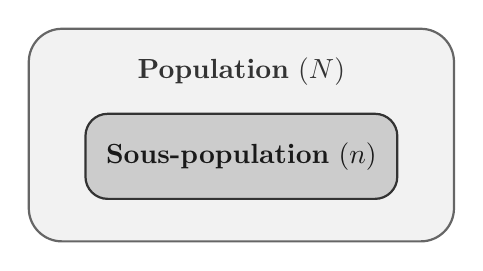
\begin{tikzpicture}[x=9mm,y=9mm]
				\draw[thick, fill=black!5, draw=black!60, rounded corners=12pt] (0,0) rectangle (6,3);
				\node[black!80] at (3, 2.4) {\textbf{Population} ($N$)};
				\draw[thick, fill=black!20, draw=black!80, rounded corners=8pt] (0.8,0.6) rectangle (5.2,1.8);
				\node[black!90] at (3, 1.2) {\textbf{Sous-population} ($n$)};
			\end{tikzpicture}
		\end{center}
		\vspace{-10mm}
	\end{wrapstuff}
	Soit $n$ l'effectif d'une sous-population incluse dans une population globale d'effectif $N$.

	La \textbf{proportion} $p$ de cette sous-population au sein de la population totale est donnée par :

	\cmath{p = \dfrac{n}{N}}
\end{df}

\begin{ex}
	\nline
	\begin{wrapstuff}[r,width=5cm]
		\begin{center}
			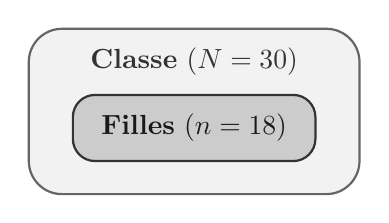
\begin{tikzpicture}[x=7mm,y=7mm]
				\draw[thick, fill=black!5, draw=black!60, rounded corners=12pt] (0,0) rectangle (6,3);
				\node[black!80] at (3, 2.4) {\textbf{Classe} ($N = 30$)};
				\draw[thick, fill=black!20, draw=black!80, rounded corners=8pt] (0.8,0.6) rectangle (5.2,1.8);
				\node[black!90] at (3, 1.2) {\textbf{Filles} ($n = 18$)};
			\end{tikzpicture}
		\end{center}
		\vspace{-15mm}
	\end{wrapstuff}
	Dans une classe de $30$ élèves, il y a $18$ filles.

	La proportion de filles dans cette classe est : $p = \dfrac{18}{30} = 0{,}6$ (soit $60$\%)
\end{ex}

\vspace{8mm}
\begin{prop}
	Une \textbf{proportion} s'exprime par un nombre compris entre $0$ et $1$ (soit entre $0\,\%$ et $100\,\%$). On a : \cmath{0 \leqslant p \leqslant 1}
\end{prop}

\begin{rmq}
	\nline
	\begin{itemize}
		\item La \textbf{proportion} est une valeur théorique ou fixe mesurée sur une population globale.
		\item La \textbf{fréquence} est le résultat d'une observation ou d'un comptage sur un échantillon donné (par exemple lors d'une expérience aléatoire ou d'un sondage).
	\end{itemize}
\end{rmq}

\begin{rmq}
	Pour retrouver les trois formules associées :
	\begin{wrapstuff}[r,width=7cm]
		\vspace{-5mm}
		\begin{center}
			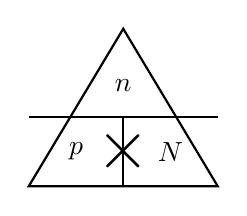
\begin{tikzpicture}[x=8mm,y=8mm]
				% Triangle principal
				\draw[thick] (0,0) -- (3,0) -- (1.5,2.5) -- cycle;
				\draw[thick] (0,1.1) -- (3,1.1);
				\draw[thick] (1.5,0) -- (1.5,1.1);
				% Labels
				\node at (1.5, 1.6) {\textbf{$n$}};
				\node at (0.75, 0.55) {\textbf{$p$}};
				\node at (2.25, 0.55) {\textbf{$N$}};
				\node at (1.5, 0.55) {\Huge$\times$};
			\end{tikzpicture}
		\end{center}
		\vspace{-10mm}
	\end{wrapstuff}
	\begin{itemize}
		\item \makebox[2cm][l]{$p = \dfrac{n}{N}$} pour calculer une proportion
		\item \makebox[2cm][l]{$n = p \times N$} pour calculer un effectif partiel
		\item \makebox[2cm][l]{$N = \dfrac{n}{p}$} pour retrouver l'effectif total
	\end{itemize}
\end{rmq}

\begin{ex}
	\nline
	\begin{enumerate}
		\item \textbf{Calculer une proportion :} Dans une entreprise de $250$ salariés, $65$ travaillent dans le service commercial.

		      \[
			      p = \dfrac{n}{N} = \dfrac{65}{250} = 0{,}26 \quad \text{soit } 26\,\%
		      \]

		      La proportion de salariés travaillant au service commercial est de $26\,\%$.

		\item \textbf{Calculer un effectif :} Dans un lycée de $1\,200$ élèves, $15\,\%$ des élèves sont inscrits en spécialité Mathématiques (soit $p = 0{,}15$).

		      \[
			      {n = p \times N = 0{,}15 \times 1\,200 = 180}
		      \]

		      Il y a $180$ élèves inscrits en spécialité Mathématiques.

		\item \textbf{Retrouver l'effectif total :} Dans un club sportif, $42$ adhérents jouent au tennis, ce qui représente $35\,\%$ de l'effectif du club ($p = 0{,}35$).

		      \[
			      N = \dfrac{n}{p} = \dfrac{42}{0{,}35} = 120
		      \]

		      Le club compte $120$ adhérents au total.
	\end{enumerate}
\end{ex}

\subsection{Proportion de proportion}

\begin{prop}
	\nline
	\begin{wrapstuff}[r,width=7.5cm]
		\begin{center}
			\begin{tikzpicture}[x=1cm,y=1cm]
				\draw[thick, fill=gray!5, draw=gray!60, rounded corners=12pt] (0,0) rectangle (7,4.5);
				\node[gray!80!black, font=\small] at (1.8, 4.1) {\textbf{Population} $E$};
				\draw[thick, fill=black!10, draw=black!60, rounded corners=10pt] (0.6,0.5) rectangle (5.2,3.4);
				\node[black!80!black, font=\small] at (2.1, 3) {\textbf{Population} $B$};
				\draw[thick, fill=black!30, draw=black!90!black, rounded corners=8pt] (1.1,0.9) rectangle (3.5,2.4);
				\node[black!90!black, font=\small] at (2.3, 1.65) {\textbf{Sous-pop.} $A$};
				\draw[->, >=Stealth, thick, black!80!black] (3.6, 1.65) -- (4.8, 1.65) node[midway, above, font=\footnotesize] {$p_1$};
				\draw[->, >=Stealth, thick, gray!80!black] (5.3, 2) -- (6.4, 2) node[midway, above, font=\footnotesize] {$p_2$};
			\end{tikzpicture}
			\vspace{-23mm}
		\end{center}
	\end{wrapstuff}

	Soit une sous-population $A$ incluse dans $B$, elle-même incluse dans une population $E$.

	Si $A$ a une proportion $p_1$ dans $B$, et $B$ a une proportion $p_2$ dans $E$, alors la proportion $p$ de $A$ dans $E$ est :

	\cmath{p = p_1 \times p_2}

\end{prop}

\vspace{12mm}

\begin{ex}
	Dans un lycée, $60\,\%$ des élèves sont en classe de Seconde (soit $p_1 = 0{,}6$).

	Parmi ces élèves de Seconde, $55\,\%$ étudient l'espagnol en LV2 (soit $p_2 = 0{,}55$).

	La proportion $p$ d'élèves de Seconde qui étudient l'espagnol dans l'ensemble du lycée est :

	\cmath{p = p_1 \times p_2 = 0{,}6 \times 0{,}55 = 0{,}33 \quad \text{(soit } 33\,\%\text{)}}

	Ainsi, $33\,\%$ des élèves du lycée sont des élèves de Seconde qui étudient l'espagnol.
\end{ex}

\begin{rmq}
	Prendre une proportion d'une autre proportion revient à les \textbf{multiplier entre elles}.

	Par exemple, calculer $50\,\%$ de $30\,\%$ revient à effectuer : $\quad 0{,}5 \times 0{,}3 = 0{,}15 \quad \text{(soit } 15\,\%\text{)}$
\end{rmq}

\section{Évolution et taux d'évolution}

\subsection{Taux d'évolution}

\begin{df}
	\nline
	\begin{wrapstuff}[r,width=6cm]
		\begin{center}
			\begin{tikzpicture}[x=1cm,y=1cm,>=Stealth]
				\node[ draw=black!80, fill=black!5, thick, rounded corners=4pt, inner sep=8pt, align=center ] (T) at (2.5,0) {Taux d'évolution\\$\pm t\,\%$};
				\node (VI) at (0,0) {$V_I$};
				\node (VF) at (5,0) {$V_F$};
				\draw[->, thick] (VI) -- (T);
				\draw[->, thick] (T) -- (VF);
			\end{tikzpicture}
		\end{center}
	\end{wrapstuff}
	Soit une grandeur passant d'une \textbf{valeur initiale} $V_I$ à une \textbf{valeur finale} $V_F$ (avec $V_I > 0$).

	Le \textbf{taux d'évolution} (ou variation relative) $t$ est donné par :

	\cmath{t = \dfrac{V_F - V_I}{V_I}}

	Pour l'exprimer en \textbf{pourcentage}, on calcule :
	\cmath{t_{\,\%} = \dfrac{V_F - V_I}{V_I} \times 100}
\end{df}

\begin{ex}
	\nline
	\begin{wrapstuff}[r,width=6cm]
		\begin{center}
			\begin{tikzpicture}[x=1cm,y=1cm,>=Stealth]
				\node[ draw=black!80, fill=black!5, thick, rounded corners=4pt, inner sep=8pt, align=center ] (T) at (2,0) {$+30\,\%$};
				\node (VI) at (0,0) {$9{,}50\eur{}$};
				\node (VF) at (4,0) {$12{,}35\eur{}$};
				\draw[->, thick] (VI) -- (T);
				\draw[->, thick] (T) -- (VF);
			\end{tikzpicture}
		\end{center}
		% \vspace{-8mm}
	\end{wrapstuff}
	Le prix d'un livre passe de $V_I = 9{,}50$\eur{} à $V_F = 12{,}35$\eur{}.

	Le taux d'évolution est :

	\cmath{t = \dfrac{12{,}35 - 9{,}50}{9{,}50} = \dfrac{2{,}85}{9{,}50} = 0{,}30}

	Le prix a donc augmenté de $30\,\%$.
\end{ex}

\begin{rmq}
	\nline
	\begin{itemize}
		\item Si le taux d'évolution $t$ est positif ($t > 0$), il s'agit d'une \textbf{augmentation}.
		\item Si le taux d'évolution $t$ est négatif ($t < 0$), il s'agit d'une \textbf{diminution}.
	\end{itemize}
\end{rmq}

\subsection{Coefficient multiplicateur}

\begin{prop}
	Augmenter ou diminuer une valeur initiale $V_I$ d'un taux de $t_{\,\%}$ revient à la multiplier par $\pa{1 + \dfrac{t}{100}}$.

	La valeur finale est alors donnée par :

	\[
		V_F = V_I \times \left( 1 + \frac{t}{100} \right)
	\]

	Le nombre $CM = \pa{1 + \dfrac{t}{100}}$ est appelé le \textbf{coefficient multiplicateur}.
	\begin{center}
		\begin{tikzpicture}[x=1cm,y=1cm,>=Stealth]
			\node[ draw=black!80, fill=black!5, thick, rounded corners=4pt, inner sep=8pt, align=center ] (T) at (3,0) {$\pm t\,\%$};
			\node (VI) at (0,0) {$V_I$};
			\node (VF) at (6,0) {$V_F$};
			\draw[->, thick] (VI) -- (T);
			\draw[->, thick] (T) -- (VF);
			\draw[->, thick, shorten >=3mm, shorten <=3mm] (VI.south) to[out=-30, in=-150] node[below=1mm] {$\times\,CM$} (VF.south);
		\end{tikzpicture}
	\end{center}
\end{prop}

\begin{demo}
	Appliquer une variation de $t\,\%$ à une valeur initiale $V_I$ consiste à ajouter (ou retrancher si $t < 0$) la partie correspondante :

	\[
		V_F = V_I + \frac{t}{100} \times V_I
	\]

	En factorisant par $V_I$, on obtient :

	\[
		V_F = V_I \times \left( 1 + \frac{t}{100} \right)
	\]
\end{demo}

\begin{ex}
	Un article coûtant $80$\eur{} subit une hausse de $15\,\%$ (soit $t = +15$).
	\begin{wrapstuff}[r,width=6cm]
		\begin{center}
			\begin{tikzpicture}[x=0.75cm,y=1cm,>=Stealth]
				\node[ draw=black!80, fill=black!5, thick, rounded corners=4pt, inner sep=6pt, align=center ] (T) at (2.5,0) {$+15\,\%$};
				\node (VI) at (0,0) {$80\text{\eur{}}$};
				\node (VF) at (5,0) {$92\text{\eur{}}$};
				\draw[->, thick] (VI) -- (T);
				\draw[->, thick] (T) -- (VF);
				\draw[->, thick, shorten >=3mm, shorten <=3mm] (VI.south) to[out=-30, in=-150] node[below=1mm] {$\times\,1{,}15$} (VF.south);
			\end{tikzpicture}
		\end{center}
		\vspace{-10mm}
	\end{wrapstuff}

	Le coefficient multiplicateur associé est :

	\cmath{CM = 1 + \dfrac{15}{100} = 1 + 0{,}15 = 1{,}15}

	Le nouveau prix $V_F$ est donc : $\quad V_F = 80 \times 1{,}15 = 92\text{\eur{}}$
\end{ex}

\begin{rmq}
	Pour une grandeur passant d'une valeur initiale $V_I$ à une valeur finale $V_F$ avec un taux d'évolution $t$ exprimé en pourcentage ($t_{\,\%}$) et un coefficient multiplicateur $CM$ :

	\begin{itemize}
		\item \makebox[4cm][l]{$t = \dfrac{V_F - V_I}{V_I} \times 100$}
		      pour calculer le taux d'évolution en pourcentage
		\item \makebox[4cm][l]{$CM = 1 + \dfrac{t}{100}$} pour obtenir le coefficient multiplicateur à partir du taux $t\,\%$
		\item \makebox[4cm][l]{$t = (CM - 1) \times 100$} pour retrouver le taux en pourcentage à partir du $CM$
	\end{itemize}

	Pour passer facilement du taux d'évolution $t\,\%$ au coefficient multiplicateur $CM$ (et inversement), on peut utiliser le petit schéma ci-dessous :

	\begin{center}
		\begin{tikzpicture}[x=1cm,y=1cm,>=Stealth]
			\node[font=\large] (T) at (0,0) {$t$};
			\node[font=\large] (M) at (3,0) {};
			\node[font=\large] (CM) at (6.5,0) {$CM$};
			\draw[->, thick,shorten >=1mm, shorten <=1mm] ([yshift=1mm]T.east) -- node[above] {$\div\,100$} ([yshift=1mm]M.west);
			\draw[->, thick,shorten >=1mm, shorten <=1mm] ([yshift=1mm]M.east) -- node[above] {$+1$} ([yshift=1mm]CM.west);

			% Trajet retour (vers la gauche, decale vers le bas)
			\draw[->, thick, shorten >=1mm, shorten <=1mm] ([yshift=-1mm]CM.west) -- node[below] {$-1$} ([yshift=-1mm]M.east);
			\draw[->, thick, shorten >=1mm, shorten <=1mm] ([yshift=-1mm]M.west) -- node[below] {$\times\,100$} ([yshift=-1mm]T.east);
		\end{tikzpicture}
	\end{center}
\end{rmq}

\begin{exo}
	Le prix d'un smartphone est initialement de $320$\eur{}. Lors d'une vente flash, ce prix subit une baisse de $15\,\%$.

	Calculer le prix final de ce smartphone après la réduction.

	\begin{correction}
		Calculons le coefficient multiplicateur correspondant à une baisse de $15\,\%$ :

		\cmath{CM = 1 + \dfrac{-15}{100} = 1 - 0{,}15 = 0{,}85}

		Calculons la valeur finale $V_F$ :

		\cmath{V_F = V_I \times CM = 320 \times 0{,}85 = 272\text{\eur{}}}

		Le prix du smartphone après réduction est donc de $272$\eur{}.
	\end{correction}
\end{exo}

\begin{exo}
	Après une augmentation de $8\,\%$, le loyer mensuel d'un appartement s'élève désormais à $648$\eur{}.

	Déterminer le montant du loyer avant cette augmentation.

	\begin{correction}
		Le coefficient multiplicateur associé à une hausse de $8\,\%$ est :

		\cmath{CM = 1 + \dfrac{8}{100} = 1{,}08}

		On cherche la valeur initiale $V_I$ telle que $V_F = V_I \times CM$, c'est-à-dire :

		\cmath{648 = V_I \times 1{,}08}

		D'où :

		\cmath{V_I = \dfrac{648}{1{,}08} = 600\text{\eur{}}}

		Le loyer avant augmentation était de $600$\eur{}.
	\end{correction}
\end{exo}

\begin{exo}
	Une étude statistique montre qu'entre deux années consécutives, le nombre de clients d'un magasin a été multiplié par un coefficient $CM = 0{,}82$.

	Déterminer le taux d'évolution exprimé en pourcentage du nombre de clients.

	\begin{correction}
		On utilise la formule reliant le coefficient multiplicateur et le taux en pourcentage :

		\cmath{t_{\,\%} = (CM - 1) \times 100}

		En remplaçant par la valeur du $CM$ :

		\cmath{t_{\,\%} = (0{,}82 - 1) \times 100 = -0{,}18 \times 100 = -18\,\%}

		Le nombre de clients a donc subi une diminution de $18\,\%$.
	\end{correction}
\end{exo}

\section{Évolutions successives et évolution réciproque}

\subsection{Évolutions successives}

\begin{prop}
	Lorsqu'une grandeur subit $n$ évolutions successives de coefficients multiplicateurs respectifs $CM_1$, $CM_2$, $\dots$, $CM_n$, le \textbf{coefficient multiplicateur global} $CM_g$ est égal au produit de tous les coefficients multiplicateurs :

	\[
		CM_g = CM_1 \times CM_2 \times \dots \times CM_n
	\]

	La valeur finale $V_F$ après ces $n$ évolutions s'obtient alors directement par : \quad $V_F = V_I \times CM_g$

	\begin{center}
		\begin{tikzpicture}[x=1cm,y=1cm,>=Stealth]
			\node (V0) at (0,0) {$V_0$};
			\node (V1) at (3.2,0) {$V_1$};
			\node (V2) at (6.4,0) {$V_2$};
			\node (Vn1) at (8.0,0) {$\phantom{I}\ldots\phantom{I}$};
			\node (Vn) at (11.2,0) {$V_n$};
			\node[ draw=black!80, fill=black!5, thick, rounded corners=4pt, inner sep=5pt, align=center ] (T1) at (1.6,0) {$t_1\,\%$};
			\node[ draw=black!80, fill=black!5, thick, rounded corners=4pt, inner sep=5pt, align=center ] (T2) at (4.8,0) {$t_2\,\%$};
			\node[ draw=black!80, fill=black!5, thick, rounded corners=4pt, inner sep=5pt, align=center ] (Tn) at (9.6,0) {$t_n\,\%$};
			\draw[->, thick] (V0) -- (T1);
			\draw[->, thick] (T1) -- (V1);
			\draw[->, thick] (V1) -- (T2);
			\draw[->, thick] (T2) -- (V2);
			\draw[->, thick, looseness=0] (V2) -- (Vn1);
			\draw[->, thick] (Vn1) -- (Tn);
			\draw[->, thick] (Tn) -- (Vn);
			\draw[->, thick, shorten >=2mm, shorten <=2mm] (V0.north) to[out=35, in=145] node[above=1mm] {$\times\,CM_1$} (V1.north);
			\draw[->, thick, shorten >=2mm, shorten <=2mm] (V1.north) to[out=35, in=145] node[above=1mm] {$\times\,CM_2$} (V2.north);
			\draw[->, thick, shorten >=2mm, shorten <=2mm] (Vn1.north) to[out=35, in=145] node[above=1mm] {$\times\,CM_n$} (Vn.north);
			\draw[->, thick, dashed, shorten <=2mm] (V2.north) to[out=35, in=180] ++(1,0.45);
			\draw[->, thick, shorten >=3mm, shorten <=3mm] (V0.south) to[out=-45, in=-135, looseness=0.35] node[below=1.5mm] {$\times\,CM_g = \times\,(CM_1 \times CM_2 \times \dots \times CM_n)$} (Vn.south);
		\end{tikzpicture}
	\end{center}
\end{prop}

\begin{ex}
	Le prix d'un vêtement de $50$\eur{} augmente d'abord de $10\,\%$, puis baisse de $20\,\%$, et augmente de $5\,\%$.
	\begin{multicols}{3}
		\begin{itemize}
			\item $CM_1 = 1 + \dfrac{10}{100} = 1{,}10$
			\item $CM_2 = 1 - \dfrac{20}{100} = 0{,}80$
			\item $CM_3 = 1 + \dfrac{5}{100} = 1{,}05$
		\end{itemize}
	\end{multicols}

	Le coefficient multiplicateur global est :

	\cmath{CM_g = CM_1 \times CM_2 \times CM_3 = 1{,}10 \times 0{,}80 \times 1{,}05 = 0{,}924}

	Le prix final du vêtement est :

	\cmath{V_F = 50 \times 0{,}924 = 46{,}20\text{\eur{}}}

	Le taux d'évolution global est :

	\cmath{t_g = (CM_g - 1) \times 100 = (0{,}924 - 1) \times 100 = -7{,}6\,\%}

	Soit une baisse globale de $7{,}6\,\%$.
\end{ex}

\begin{erreur}
	On ne peut pas additionner ni soustraire directement les pourcentages d'évolutions successives !

	Par exemple, une hausse de $20\,\%$ suivie d'une baisse de $20\,\%$ \textbf{ne correspond pas} à une variation nulle ($0\,\%$).

	En effet :
	\begin{multicols}{2}
		\begin{itemize}
			\item Hausse de $20\,\%$ : \quad $CM_1 = 1 + \dfrac{20}{100} = 1{,}20$
			\item Baisse de $20\,\%$ : \quad $CM_2 = 1 - \dfrac{20}{100} = 0{,}80$
		\end{itemize}
	\end{multicols}

	On a : \cmath{CM_g = 1{,}20 \times 0{,}80 = 0{,}96}

	Le taux global est : \cmath{t_g = (0{,}96 - 1) \times 100 = -4\,\%}

	L'évolution globale est donc une \textbf{baisse de $4\,\%$}.

	Pour compenser exactement une hausse de $20\,\%$ et revenir à la valeur initiale, la baisse réciproque doit être différente de $20\,\%$.
\end{erreur}

\subsection{Évolution réciproque}

\begin{defn}
	\nline
	\begin{wrapstuff}[r, width=7cm]
		\begin{center}
			\vspace{5mm}
			\begin{tikzpicture}[x=1cm,y=1cm,>=Stealth]
				\node (VI1) at (0,0) {$V_I$};
				\node (VF) at (2.8,0) {$V_F$};
				\node (VI2) at (5.6,0) {$V_I$};
				\node[ draw=black!80, fill=black!5, thick, rounded corners=4pt, inner sep=5pt, minimum width=1cm, align=center ] (T) at (1.4,0) {$t$};
				\node[ draw=black!80, fill=black!5, thick, rounded corners=4pt, inner sep=5pt, minimum width=1cm, align=center ] (TR) at (4.2,0) {$t_R$};
				\draw[->, thick] (VI1) -- (T);
				\draw[->, thick] (T) -- (VF);
				\draw[->, thick] (VF) -- (TR);
				\draw[->, thick] (TR) -- (VI2);
			\end{tikzpicture}
			\vspace{1mm}
		\end{center}
	\end{wrapstuff}

	On considère une grandeur subissant une évolution d'une valeur initiale $V_I$ vers une valeur finale $V_F$.

	L'\textbf{évolution réciproque} est l'évolution qui permet de revenir de la valeur finale $V_F$ à la valeur initiale $V_I$.

	Elle compense exactement la variation subie lors de l'évolution initiale.

	Son taux d'évolution est appelé \textbf{taux d'évolution réciproque}, noté $t_R$.
\end{defn}

\begin{prop}
	\nline
	\begin{wrapstuff}[r, width=7cm]
		\begin{center}
			\vspace{5mm}
			\begin{tikzpicture}[x=1cm,y=1cm,>=Stealth]
				% Nœuds des valeurs
				\node (VI1) at (0,0) {$V_I$};
				\node (VF) at (2.8,0) {$V_F$};
				\node (VI2) at (5.6,0) {$V_I$};

				% Boîtes de taux
				\node[ draw=black!80, fill=black!5, thick, rounded corners=4pt, inner sep=5pt, minimum width=1cm, align=center ] (T) at (1.4,0) {$t$};
				\node[ draw=black!80, fill=black!5, thick, rounded corners=4pt, inner sep=5pt, minimum width=1cm, align=center ] (TR) at (4.2,0) {$t_R$};

				% Flèches horizontales
				\draw[->, thick] (VI1) -- (T);
				\draw[->, thick] (T) -- (VF);
				\draw[->, thick] (VF) -- (TR);
				\draw[->, thick] (TR) -- (VI2);

				% Arcs sous les boîtes (CM et CMR)
				\draw[->, thick, shorten >=2mm, shorten <=2mm] (VI1.south) to[out=-35, in=-145] node[below=1mm, font=\small] {$\times\,CM$} (VF.south);
				\draw[->, thick, shorten >=2mm, shorten <=2mm] (VF.south) to[out=-35, in=-145] node[below=1mm, font=\small] {$\times\,CM_R$} (VI2.south);
			\end{tikzpicture}
		\end{center}
	\end{wrapstuff}

	Soit une évolution de taux $t$ et son coefficient multiplicateur associé $CM$.

	L'évolution réciproque, de taux $t_R$, possède un \textbf{coefficient multiplicateur réciproque}, noté $CM_R$, vérifiant la relation :

	\cmath{CM_R = \dfrac{1}{CM}}

	Le taux d'évolution réciproque s'obtient ensuite par : \qquad $t_R = (CM_R - 1) \times 100$
\end{prop}

\begin{demo}
	Par définition de l'évolution réciproque, le coefficient $CM_R$ permet de revenir de $V_F$ à $V_I$ :

	\[
		\def\arraystretch{1.7} \begin{array}{rrcll}
			     & V_F & = & V_I \times CM                                                                  \\
			\iff & V_I & = & \dfrac{V_F}{CM}          & \text{(on isole } V_I\text{)}                       \\
			\iff & V_I & = & V_F \times \dfrac{1}{CM} & \text{(diviser revient à multiplier par l'inverse)}
		\end{array}
	\]

	Par identification avec la relation $V_I = V_F \times CM_R$, on en déduit immédiatement : \quad $CM_R = \dfrac{1}{CM}$
\end{demo}

\begin{exemple}
	Un article subit une hausse de $20\,\%$. On cherche à déterminer le taux de l'évolution réciproque $t_R$ permettant de revenir au prix initial.

	\begin{enumerate}
		\item {Calcul du coefficient multiplicateur initial :}
		      \[
			      CM = 1 + \frac{20}{100} = 1{,}20
		      \]
		\item {Calcul du coefficient multiplicateur réciproque :}
		      \[
			      CM_R = \frac{1}{CM} = \frac{1}{1{,}20} = \frac{5}{6} \approx 0{,}8333
		      \]
		\item {Calcul du taux d'évolution réciproque :}
		      \[
			      t_R = (CM_R - 1) \times 100 = \left( \frac{5}{6} - 1 \right) \times 100 = -\frac{100}{6} \approx -16{,}67\,\%
		      \]
	\end{enumerate}

	Pour compenser une hausse de $20\,\%$, il faut donc effectuer une baisse d'environ $16{,}67\,\%$.
\end{exemple}

\newpage

\begin{exercice}
	Un laboratoire étudie l'évolution d'une population de \textbf{licornes magiques} dans une forêt enchantée sur trois années consécutives.

	\begin{itemize}
		\item La $1\iere$ année, suite à une surconsommation d'arcs-en-ciel, la population \textbf{augmente de $25\,\%$}.
		\item La $2\ieme$ année, en raison d'une pénurie de paillettes, la population \textbf{chute de $40\,\%$}.
		\item La $3\ieme$ année, grâce à une récolte exceptionnelle d'herbe dorée, la population \textbf{augmente de $50\,\%$}.
	\end{itemize}

	\begin{enumerate}
		\item Déterminer le coefficient multiplicateur associé à chaque évolution annuelle ($CM_1$, $CM_2$ et $CM_3$).
		\item En déduire le coefficient multiplicateur global $CM_g$ sur ces trois années.
		\item Calculer le taux d'évolution global $t_g$ de la population de licornes sur cette période.\\
		      La population a-t-elle augmenté ou diminué au global ?
		\item Le garde forestier souhaite ramener la population de licornes exactement à son niveau initial.
		      \begin{enumerate}
			      \item Calculer le coefficient multiplicateur réciproque $CM_R$.
			      \item En déduire le taux d'évolution réciproque $t_R$ (arrondi au centième près) à appliquer à la population finale.
		      \end{enumerate}
	\end{enumerate}

	\begin{correction}
		\nline
		\begin{enumerate}
			\item {Coefficients multiplicateurs annuels :}
			      \begin{multicols}{3}
				      \begin{itemize}
					      \item $CM_1 = 1 + \dfrac{25}{100} = 1{,}25$
					      \item $CM_2 = 1 + \dfrac{-40}{100} = 0{,}60$
					      \item $CM_3 = 1 + \dfrac{50}{100} = 1{,}50$
				      \end{itemize}
			      \end{multicols}

			\item {Coefficient multiplicateur global :}
			      \[
				      CM_g = CM_1 \times CM_2 \times CM_3 = 1{,}25 \times 0{,}60 \times 1{,}50 = 1{,}125
			      \]

			\item {Taux d'évolution global :}
			      \[
				      t_g = (CM_g - 1) \times 100 = (1{,}125 - 1) \times 100 = +12{,}5\,\%
			      \]
			      Sur les trois années, la population de licornes a subi une \textbf{hausse globale de $12{,}5\,\%$}.

			\item {Évolution réciproque :}
			      \begin{enumerate}
				      \item {Coefficient multiplicateur réciproque :}
				            \[
					            CM_R = \frac{1}{CM_g} = \frac{1}{1{,}125} = \frac{8}{9} \approx 0{,}8889
				            \]

				      \item {Taux d'évolution réciproque :}
				            \[
					            t_R = (CM_R - 1) \times 100 = \left( \frac{8}{9} - 1 \right) \times 100 = \frac{-100}{9} \approx -11{,}11\,\%
				            \]
				            Pour revenir exactement à la population initiale, il faut appliquer une \textbf{baisse d'environ $11{,}11\,\%$}.
			      \end{enumerate}
		\end{enumerate}
	\end{correction}
\end{exercice}
